\documentclass[10pt,a4paper,ngerman,oneside,]{article}
\newcommand\teamname{Lühack}
\newcommand\teammembers{Lennart Weckeck\\ Thore Tiemann\\ Marcel Wienöbst}
\newcommand\university{Universität zu Lübeck}

\usepackage[log-declarations=false]{xparse}
\usepackage[utf8]{luainputenc}
\usepackage{luacode}
\usepackage[T1]{fontenc}
\usepackage{fontspec}
\usepackage[english]{babel}

\defaultfontfeatures{Ligatures=TeX}
\setmainfont{TeX Gyre Termes}
\setmonofont{Source Code Pro}

\usepackage[unicode,pdfencoding=auto,hidelinks]{hyperref}
\setlength{\columnseprule}{0.25pt}
\linespread{1.180}
\usepackage[left=1.5cm,right=.75cm,top=2.0cm,bottom=.8cm]{geometry}

\usepackage{fancyhdr}
\usepackage{lastpage}
\pagestyle{fancy}
\fancyhf{}
\fancyhead[R]{ACM ICPC Reference, page \bfseries\thepage/\pageref{LastPage}}
\fancyhead[L]{\university, Team: \teamname}

\usepackage{mathtools}
\usepackage{amsfonts}
\usepackage{amssymb}
\newcommand{\N}{\ensuremath{\mathbb{N}}}
\renewcommand{\C}{\ensuremath{\mathbb{C}}}
\newcommand{\lcm}{\ensuremath{\operatorname{lcm}}}
\newcommand{\bigo}[1]{\text{$\mathcal{O}\left(#1\right)$}}

\usepackage{algorithm}
\usepackage{algorithmic}

\usepackage{graphicx}
\usepackage{pdfpages}
\usepackage{xcolor}
\definecolor{darkgreen}{rgb}{0,0.5,0}
\definecolor{uni}{RGB}{0,75,90}

\usepackage{listings}
\lstset{numbers=left,
        captionpos=b,
        emptylines=*1,
%        language=Java,
        numberstyle=\ttfamily\tiny,
        basicstyle=\ttfamily\footnotesize,
        identifierstyle=\color{black},
        keywordstyle=\ttfamily\bfseries\color{uni},
        commentstyle=\color{darkgreen},
        stringstyle=\color{violet},
        backgroundcolor=\color{black!5},
        frame=lines,
        framerule=1.0pt,
        showspaces=false,
        showtabs=false,
        tabsize=2,
        numbersep=5pt,
        mathescape=true,
        breaklines=true,
        % breakatwhitespace=true,
        % prebreak=\raisebox{0ex}[0ex][0ex]{\ensuremath{\space\color{red}\rhookswarrow}},
        % postbreak=\raisebox{0ex}[0ex][0ex]{\ensuremath{\color{red}\hookrightarrow\space}}
}
\usepackage{multicol}
\setlength{\parindent}{0pt}

\newenvironment{java}{%
    % variables
    \def\algorithmName{\color{red}Title not set}%
    \def\algorithmDescription{\color{red}Description not set}%
    \def\algorithmFile{No File given}%
    \def\algorithmComplexity{?}%
    \def\algorithmHash{-}%
    \def\algorithmLanguage{Java}%
    % setter
    \newcommand{\setAlgorithmName}[1]{\def\algorithmName{##1}}%
    \newcommand{\setAlgorithmDescription}[1]{\def\algorithmDescription{##1}}%
    \newcommand{\setAlgorithmFile}[1]{\def\algorithmFile{##1}}%
    \newcommand{\setAlgorithmComplexity}[1]{\def\algorithmComplexity{##1}}%
    \newcommand{\setAlgorithmHash}[1]{\def\algorithmHash{##1}}%
}{%
    \subsection{\algorithmName}%
    \algorithmDescription%
    \lstinputlisting[title=
    {\footnotesize{\textbf{MD5:}\;\texttt{\algorithmHash}\;\mid\;%
    $\mathcal{O}(\algorithmComplexity)$}},language=Java]{\algorithmFile}%
}%

\newenvironment{cpp}{%
    % variables
    \def\algorithmName{\color{red}Title not set}%
    \def\algorithmDescription{\color{red}Description not set}%
    \def\algorithmFile{No File given}%
    \def\algorithmComplexity{?}%
    \def\algorithmHash{-}%
    \def\algorithmLanguage{Java}%
    % setter
    \newcommand{\setAlgorithmName}[1]{\def\algorithmName{##1}}%
    \newcommand{\setAlgorithmDescription}[1]{\def\algorithmDescription{##1}}%
    \newcommand{\setAlgorithmFile}[1]{\def\algorithmFile{##1}}%
    \newcommand{\setAlgorithmComplexity}[1]{\def\algorithmComplexity{##1}}%
    \newcommand{\setAlgorithmHash}[1]{\def\algorithmHash{##1}}%
}{%
    \subsection{\algorithmName}%
    \algorithmDescription%
    \lstinputlisting[title=
    {\footnotesize{\textbf{MD5:}\;\texttt{\algorithmHash}\;\mid\;%
    $\mathcal{O}(\algorithmComplexity)$}},language=C++]{\algorithmFile}%
}%

\newenvironment{python}{%
    % variables
    \def\algorithmName{\color{red}Title not set}%
    \def\algorithmDescription{\color{red}Description not set}%
    \def\algorithmFile{No File given}%
    \def\algorithmComplexity{?}%
    \def\algorithmHash{-}%
    \def\algorithmLanguage{Java}%
    % setter
    \newcommand{\setAlgorithmName}[1]{\def\algorithmName{##1}}%
    \newcommand{\setAlgorithmDescription}[1]{\def\algorithmDescription{##1}}%
    \newcommand{\setAlgorithmFile}[1]{\def\algorithmFile{##1}}%
    \newcommand{\setAlgorithmComplexity}[1]{\def\algorithmComplexity{##1}}%
    \newcommand{\setAlgorithmHash}[1]{\def\algorithmHash{##1}}%
}{%
    \subsection{\algorithmName}%
    \algorithmDescription%
    \lstinputlisting[title=
    {\footnotesize{\textbf{MD5:}\;\texttt{\algorithmHash}\;\mid\;%
    $\mathcal{O}(\algorithmComplexity)$}},language=Python]{\algorithmFile}%
}%

\title{Team Contest Reference}
\author{\university}

\begin{document}
\vspace{-5mm}
\begin{center}
	\begin{minipage}{0.3\textwidth}
	  
\includegraphics[scale=.8,clip,trim=.4cm 0cm 6.4cm 0cm,scale=0.89]{img/logo_uzl.pdf}
    \end{minipage}
	\begin{minipage}{0.35\textwidth}
      \begin{center}
	    \LARGE{\bfseries Team Contest Reference}\\
        \textbf{Team:} {\teamname}
      \end{center}
    \end{minipage}
	\begin{minipage}{0.3\textwidth}
      \flushright
      \itshape\teammembers
    \end{minipage}
\end{center}
\thispagestyle{fancy}
\tableofcontents

\begin{multicols}{2}
% \vfill
\vspace{1em}{\centering
\hfill\begin{tabular}{rl}
	\hline $n$ & Runtime $100\cdot 10^{6}$ in $3$s \\\hline
	$[10,11]$ & $\mathcal{O}(n!)$ \\
	$<22$ & $\mathcal{O}(n2^n)$ \\
	$\leq 100$ & $\mathcal{O}(n^4)$ \\
	$\leq 400$ & $\mathcal{O}(n^3)$ \\
	$\leq 2.000$ & $\mathcal{O}(n^2\log n)$ \\
	$\leq 10.000$ & $\mathcal{O}(n^2)$ \\
	$\leq 1.000.000$ & $\mathcal{O}(n\log n)$ \\
	$\leq 100.000.000$ & $\mathcal{O}(n)$ \\\hline
\end{tabular}\hfill}

\vspace{1em}
\noindent
\texttt{byte} (8 Bit, signed): -128 \dots 127\\
\texttt{short} (16 Bit, signed): -32.768 \dots 23.767\\
\texttt{integer} (32 Bit, signed): -2.147.483.648 \dots 2.147.483.647\\
\texttt{long} (64 Bit, signed): $-2^{63}$\dots $2^{63}-1$\\

\newcommand{\hash}[1]{{\bfseries MD5:} ~\texttt{#1}}
\vspace{1.2em}\noindent {\textbf{MD5:}} \texttt{\small cat <string>| tr -d [:space:] | md5sum}\\

% \newpage
% \begin{multicols}{2}
\luadirect{ require('parseCode.lua') }
\luadirect{ removeTmpFiles() }
\luadirect{ parse() }
\luadirect{ removeTmpFiles() }
% \newpage
% \end{multicols}

\section{Math}
\subsection{Tree}
Diameter: BFS from any node, then BFS from last visited node.
Max dist is then the diameter.
Center: Middle vertex in second step from above.
\subsection{Divisability Explanation}
$D \mid M \Leftrightarrow D \mid {\tt digit\_sum(M, k, alt)}$, refer to table for values of $D, k, alt$.
\begin{table}[htbp]
\begin{tabular}{| c || c | c | c | c | c | c | c | c | c | c |}
\hline
$D$ & 3 & 7 & 9 & 11 & 13 & 17 & 19 & 23 & 37 & 41 \\
\hline
$k$ & 1 & 3 & 1 & 2 & 3 & 8 & 9 & 11 & 3 & 5 \\
\hline
$alt$ & f & w & f & f & w & w & w & w & f & f \\ 
\hline
\end{tabular}
\end{table}
\subsection{Combinatorics}
\begin{itemize}
\item Variations (ordered): $k$ out of $n$ objects {\footnotesize (permutations for $k = n$)}
\begin{itemize}
	\item without repetition:\\ $M = \{ (x_{1}, \ldots , x_{k}): 1 \leq x_i \leq n, \ x_i \neq x_j \mbox{ if } i \neq j \}$, $|M|= \frac{n!}{(n-k)!}$
	\item with repetition:\\ $M = \{ (x_{1}, \ldots , x_{k}): 1 \leq x_i \leq n \}, |M| = n^k$
	\end{itemize}
\item Combinations (unordered): $k$ out of $n$ objects
\begin{itemize}
	\item without repetition: $M = \{ (x_{1}, \ldots , x_{n}): x_i \in \{0,1\}, \ x_1 + \ldots + x_n = k \}$, $|M| = {n \choose k}$
	\item with repetition: $M = \{ (x_{1}, \ldots , x_{n}): x_i \in \{0,1,\ldots,k\}, \ x_1 + \ldots + x_n = k \}$, $|M| = {n+k-1 \choose k}$
\end{itemize}
\item Ordered partition of numbers: $x_1+\ldots+x_k = n$ {\footnotesize (i.e. 1+3 = 3+1 = 4 are counted as 2 solutions)}
\begin{itemize}
	\item \#Solutions for $x_i \in \mathbb{N}_0$: ${n+k-1 \choose k-1}$
	\item \#Solutions for $x_i \in \mathbb{N}$: ${n-1 \choose k-1}$
\end{itemize}
\item Unordered partition of numbers: $x_1+\ldots+x_k = n$ {\footnotesize (i.e. 1+3 = 3+1 = 4 are counted as 1 solution)}
\begin{itemize}
	\item \#Solutions for $x_i \in \mathbb{N}$: $P_{n,k} = P_{n-k,k}+P_{n-1,k-1}$ where $P_{n,1} = P_{n,n} = 1$
\end{itemize}
\item Derangements {\footnotesize (permutations without fixed points)}: $!n = n! \sum\nolimits_{k = 0}^n \frac{(-1)^k}{k!} = \lfloor \frac{n!}{e} + \frac{1}{2} \rfloor$
\end{itemize}
\subsection{Polynomial Interpolation}
\subsubsection{Theory}
Problem: for $\{(x_0,y_0),\ldots, (x_n, y_n) \}$ find $p \in \Pi_{n}$ with $p(x_i) = y_i$ for all $i=0,\ldots,n$.\\
Solution: $p(x) = \sum\limits_{i=0}^n \gamma_{0,i} \prod\limits_{j=0}^{i-1} (x-x_i)$ where $\gamma_{j,k} = y_j$ for $k = 0$ and $\gamma_{j,k} = \frac { \gamma_{j+1,k-1} - \gamma_{j,k-1} }{x_{j+k}-x_j}$ otherwise. \\
Efficient evaluation of $p(x)$: $b_n = \gamma_{0,n}$, $b_i = b_{i+1}(x-x_i) + \gamma_{0,i}$ for $i=n-1,\ldots,0$ with $b_0 = p(x)$.
\subsection{Fibonacci Sequence}
\subsubsection{Binet's formula}
$
\begin{pmatrix}
f_n \\
f_{n+1}
\end{pmatrix} =
\begin{pmatrix}
0 & 1 \\
1 & 1
\end{pmatrix}^n
\begin{pmatrix}
0 \\
1
\end{pmatrix}
\Rightarrow
f_n = \frac{1}{\sqrt{5}} (\phi^n - \tilde{\phi}^n)$ where $\phi = \frac{1+\sqrt{5}}{2}$ and $\tilde{\phi} = \frac{1-\sqrt{5}}{2}$.
\subsubsection{Generalization}
$g_n = \frac{1}{\sqrt{5}} (g_0 (\phi^{n-1} - \tilde{\phi}^{n-1}) + g_1 (\phi^n - \tilde{\phi}^n)) = g_0 f_{n-1} + g_1 f_n$ for all $g_0, g_1 \in \mathbb{N}_0$

\subsubsection{Pisano Period}
Both $(f_n \bmod k)_{n \in \mathbb{N}_0}$ and $(g_n \bmod k)_{n \in \mathbb{N}_0}$ are periodic.
\begin{table}[htbp]
\begin{tabular}{| c || c | c | c | c | c | c | c | c | c | c | c | }
\hline
$k$ & 2 & 3 & 4 & 5 & 6 & 7 & 8 & 9 & 10 & 100 & $10^n$ for $n >2$ \\
\hline
$\pi(k)$ & 3 & 8 & 6 & 20 & 24 & 16 & 12 & 24 & 60 & 300 & $15 \cdot 10^{n-1}$ \\
\hline
\end{tabular}
\end{table}

% % % % % % % % % % % % % % % % % % % % % % % % % % % % % % % % % % % % % % % % % % % % % % % % % % % % % % % % % % % % % % % % % % % % % % %
% % % % % % % % % % % % % % % % % % % % % % % % % % % % % % % % % % % % % % % % % % % % % % % % % % % % % % % % % % % % % % % % % % % % % % %
\subsection{Reihen}
$
\sum\limits_{i=1}^{n}i=\frac{n(n+1)}{2}, \sum\limits_{i=1}^{n}i^2=\frac{n(n+1)(2n+1)}{6}, \sum\limits_{i=1}^{n}i^3=\frac{n^2(n+1)^2}{4}
$\\
$
\sum\limits_{i=0}^{n}c^i=\frac{c^{n+1}-1}{c-1},c\neq 1, \sum\limits_{i=0}^{\infty}c^i=\frac{1}{1-c}, \sum\limits_{i=1}^{n}c^i=\frac{c}{1-c},|c|<1
$\\
$
\sum\limits_{i=0}^{n}ic^i=\frac{nc^{n+2}-(n+1)c^{n+1}+c}{(c-1)^2}, c\neq 1, \sum\limits_{i=0}^{\infty}ic^i=\frac{c}{(1-c)^2}, |c|<1
$

\subsection{Binomialkoeffizienten}
$
{n \choose k} = {n-1 \choose k} + {n-1 \choose k-1}
$,
$
{n \choose m}{m \choose k} = {n \choose k}{n-k \choose m-k}
$,
$
{m+n \choose r} = \sum_{k=0}^r {m \choose k}{n \choose r-k}
$ and in general,
$
{n_1 + \cdots + n_p} = \sum_{k_1 + \cdots + k_p = m} {n_1 \choose k_1}
\cdots {n_p \choose k_p}
$
\subsection{Catalanzahlen}
$
C_n=\frac{1}{n+1}\binom{2n}{n}=\frac{(2n)!}{(n+1)!n!}
$\\
$
C_0=1, C_{n+1}=\sum\limits_{k=0}^{n}C_kC_{n-k}, C_{n+1}=\frac{4n+2}{n+2}C_n
$

\subsection{Geometrie}
\textbf{Polygonfläche:} $A=\frac{1}{2}(x_1y_2-x_2y_1+x_2y_3-x_3y_2+\dots+x_{n-1}y_n-x_ny_{n-1}+x_ny_1-x_1y_n)$


\subsection{Zahlentheorie}
\textbf{Chinese Remainder Theorem:} Es existiert eine Zahl $C$, sodass:\\
$
C\equiv a_1\mod n_1,\cdots, C\equiv a_k\mod n_k, \mathrm{ggt}(n_i,n_j)=1,i\neq j
$\\
Fall $k=2$: $m_1n_1+m_2n_2=1$ mit EEA finden.\\
Lösung ist $x=a_1m_2n_2+a_2m_1n_1$.\\
Allgemeiner Fall: iterative Anwendung von $k=2$

\textbf{Eulersche $\varphi$-Funktion:} $\varphi(n)=n\prod_{p|n}(1-\frac{1}{p}),p$ prim\\
$\varphi(p)=p-1,\varphi(pq)=\varphi(p)\varphi(q)$, $p,q$ prim\\
$\varphi(p^k)=p^k-p^{k-1},p,q$ prim, $k\geq 1$

\textbf{Eulers Theorem:} $a^{\varphi(n)}\equiv 1\mod n$

\textbf{Fermats Theorem:} $a^{p}\equiv a\mod p, p$ prim

\subsection{Faltung}
$
(f\ast g)(n) = \sum\limits_{m=-\infty}^{\infty}f(m)g(n-m)=\sum\limits_{m=-\infty}^{\infty}f(n-m)g(m)
$


% % % % % % % % % % % % % % % % % % % % % % % % % % % % % % % % % % % % % % % % % % % % % % % % % % % % % % % % % % % % % % % % % % % % % % %
% % % % % % % % % % % % % % % % % % % % % % % % % % % % % % % % % % % % % % % % % % % % % % % % % % % % % % % % % % % % % % % % % % % % % % %


\section{Java Knowhow}
\subsection{System.out.printf() und String.format()}
\textbf{Syntax}: \texttt{\%[flags][width][.precision][conv]}

\textbf{flags}: \\ \begin{tabular}{ll}
  \texttt{-} & left-justify (default: right) \\
  \texttt{+} & always output number sign \\
  \texttt{0} & zero-pad numbers \\
  (space)    & space instead of minus for pos. numbers \\
  \texttt{,} & group triplets of digits with ,
\end{tabular}

\textbf{width} specifies output width

\textbf{precision} is for floating point precision

\textbf{conv}: \\ \begin{tabular}{ll}
  d & byte, short, int, long \\
  f & float, double \\
  c & char (use C for uppercase) \\
  s & String (use S for all uppercase)
\end{tabular}

\subsection{Modulo: Avoiding negative Integers}
\begin{lstlisting}
int mod = (((nums[j] % D) + D) % D);
\end{lstlisting}

\subsection{Speed up IO}
Use
\begin{lstlisting}
BufferedReader br = new BufferedReader(new
InputStreamReader(System.in));
\end{lstlisting}
Use
\begin{lstlisting}
Double.parseDouble(Scanner.next());
\end{lstlisting}
\end{multicols}

%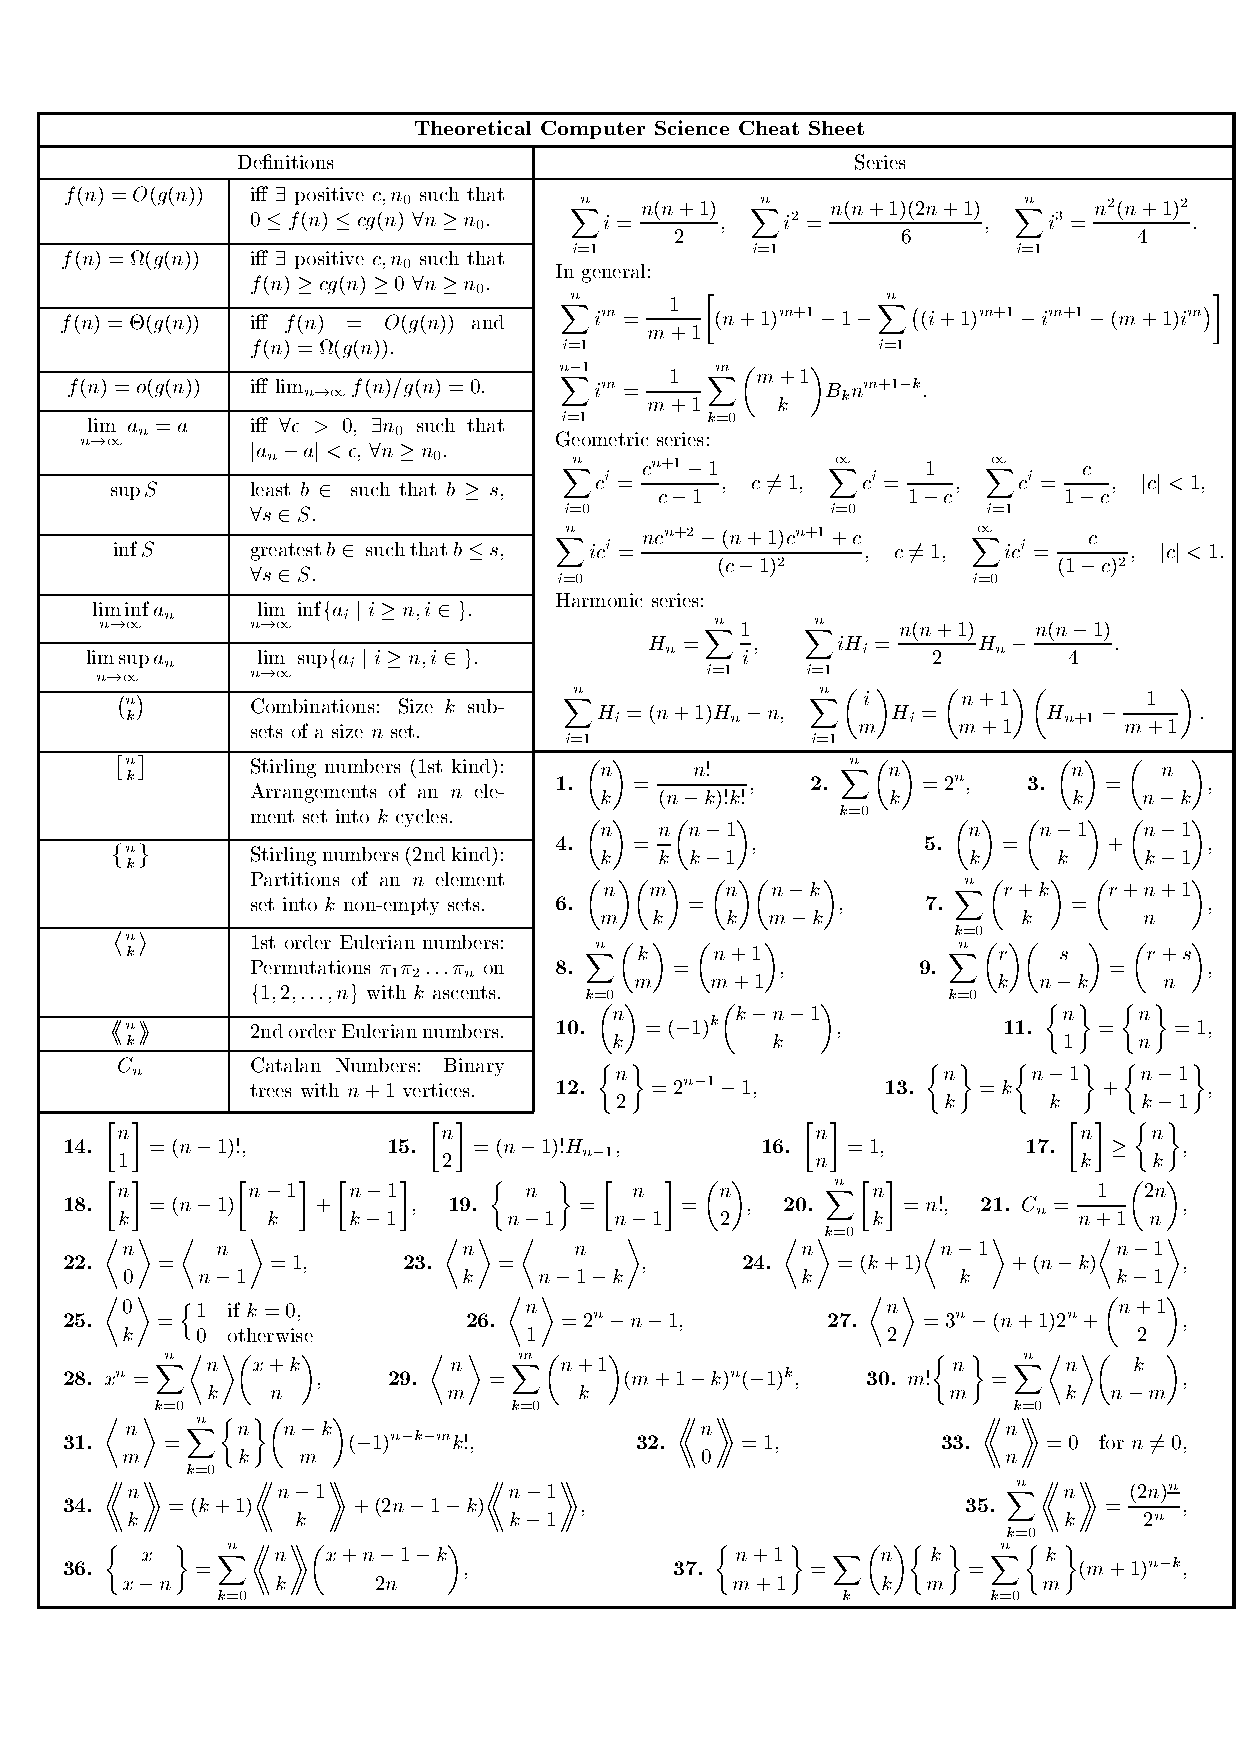
\includepdf[pages=-,clip,trim=5mm 17mm 0mm 17mm,scale=0.95,pagecommand={\pagestyle{plain}}]{tcs-cheat-sheet.pdf}

\end{document}
